\subsection{Preprocessing and Data Augmentation}

To implement the methods based on Machine learning or deep learning for hate speech detection on Twitter, a thorough data preprocessing procedure was carried out to balance the classes in the dataset. First, the two target categories were identified: \textit{hate speech} and \textit{no hate speech}, encoded as 1 and 0, respectively. Various text cleaning techniques were then applied, including the removal of special characters, URLs, mentions, Twitter-specific symbols, spelling correction, stopword removal, stemming, as well as the elimination of duplicate records and null values. Additionally, the vocabulary was enriched through synonym validation and expansion. To address the inherent class imbalance, the Easy Data Augmentation (EDA) technique was applied, which allowed for the generation of a balanced dataset, ultimately saved in a CSV file named \texttt{balanced\_data.csv}~\cite{wei2019eda}.

The preprocessing approach adopted in this study shares several similarities with previous works such as those by Fieri et al.~\cite{fieri2023offensive} and Almeida et al.~\cite{almeida2023comparison}, particularly in terms of text data cleaning and preparation for hate speech detection tasks. As in these studies, common techniques were applied, including the removal of textual noise (mentions, URLs, symbols), lexical normalization, and dimensionality reduction through the use of stopwords and stemming. However, our approach integrates additional steps that are not consistently addressed in those works, such as automated spelling correction, semantic validation using synonyms, and the application of data augmentation techniques like Easy Data Augmentation (EDA). This last aspect represents a significant difference, as the reviewed studies often rely on direct undersampling or oversampling, whereas our methodology emphasizes the synthetic generation of new samples. This can contribute to greater dataset diversity and model robustness during training, regardless of the architecture employed~\cite{wei2019eda}.


\subsection{Machine learning Methods}

\subsubsection{Methodology XGBoost}

The methodology used for the XGBoostClassifier began by loading the [CLS] token embeddings generated by RoBERTa, that is, the vector that summarizes the entire text sequence. After this, the data was split into 80\% for training and 20\% for testing. This split resulted in 38,152 examples available for training. Subsequently, a parameter grid was defined to conduct hyperparameter tuning. The search focused on the number of estimators, maximum tree depth, and minimum child weight. To find the best values, a grid search with 3-fold cross-validation was used.

In addition to this search, other hyperparameters were set manually. For example, 80\% of the data was used in each boosting round, and in each tree and node, a sample of features was selected such that its size was proportional to the square root of the total number of features, as recommended in \cite{Chen2016XGBoost}.

For training, 50\% of the dataset was used to perform the hyperparameter search, as doing it on the entire training set would have been computationally too expensive. Once the best hyperparameters were found, the model was trained on the full training set and then evaluated.

To evaluate the model, a classification report was generated that measured precision, recall, F1-score, and accuracy. Additionally, a confusion matrix was presented to more clearly observe the trend of the data toward true positives or misclassification.


\subsubsection{Logistic Regression Methodology}
To evaluate logistic regression, we first loaded the model and used the balanced dataset to compute the mean embedding of each text input. The model was then trained using these representations. The data was split into 80\% for training and 20\% for testing, and the corresponding evaluation metrics were generated.


\subsubsection{SVM}

The methodology used for SVM was very similar to the one applied with \texttt{XGBoostClassifier}. To begin with, the RoBERTa-generated embeddings were loaded. Secondly, the data was split into training and testing sets, with 80\% and 20\% of the data respectively. Then, a parameter grid was defined to conduct hyperparameter tuning. The hyperparameters tested were the kernel and \texttt{C} (penalty for misclassification). The values tested for the kernel were: \texttt{linear}, \texttt{poly}, \texttt{RBF}, and \texttt{sigmoid}; whereas for \texttt{C}, the values tested were: 0.1, 1, and 5. Finally, a grid search with 3-fold cross-validation was used.

Due to the severe computational cost of hyperparameter search, approximately 20\% of the dataset was used to perform the tuning.

To evaluate the model, F1-score, precision, recall, and accuracy were measured using a classification report. Lastly, a confusion matrix was displayed to observe how the data was being classified by the model.

\subsection{Deep Learning Methods}

\subsubsection{CNN Methodology}
\label{sec:cnn}

Using the Convolutional Neural Network (CNN) architecture, various configurations were explored to obtain an effective training setup. With a balanced dataset of 47,706 labeled messages now available, the data was split into two subsets: 80\% for training and 20\% for testing. The final model was structured with three hidden convolutional layers. Although deeper architectures were initially tested, they were deemed suboptimal given the relatively limited size of the dataset.

Each of the convolutional layers was followed by a ReLU (Rectified Linear Unit) activation function. ReLU is commonly used in deep learning because it introduces non-linearity by outputting zero for all negative values and keeping positive values unchanged, which helps avoid vanishing gradient problems and accelerates convergence.

To reduce the spatial dimensions and computational complexity of the model, a \texttt{MaxPooling1D} layer with a pool size of 2 was applied after each convolution. Max pooling extracts the most prominent feature within each segment of the input, effectively downsampling the representation and providing translation invariance, which is particularly useful in textual pattern recognition.

In order to prevent overfitting—an issue often encountered when training deep networks on relatively small datasets—Dropout layers with a dropout rate of 0.3 were included. Dropout randomly deactivates a fraction of neurons during training, which helps the model generalize better by discouraging co-adaptations of feature detectors.

Finally, the architecture concluded with a dense output layer using the sigmoid activation function. This function maps the output to a probability between 0 and 1, suitable for binary classification tasks like distinguishing between hate and non-hate speech.

The model was compiled and trained using the Adam optimizer, which combines the advantages of both AdaGrad and RMSProp by adapting the learning rate for each parameter. A learning rate of 0.0005 was selected to balance the speed of convergence with training stability, allowing the model to make gradual improvements without overshooting minima.

The implemented CNN model consists of three convolutional blocks followed by max pooling and dropout layers. This structure enables the progressive extraction of textual features while controlling overfitting. The Conv1D layers increase in complexity (from 64 to 256 filters), while MaxPooling1D reduces the dimensionality of the text, making processing more efficient.

The use of Dropout layers between convolutional blocks, with a dropout rate of 0.3, effectively mitigates overfitting—an important consideration given the dataset size of 47,706 samples. Subsequently, a Flatten layer transforms the three-dimensional output into a vector, which is then processed by a dense layer of 128 neurons. This dense layer accounts for the majority of the model’s parameters. Finally, a Dense output layer with a sigmoid activation function performs the binary classification.

Compared to previous studies such as those by Fieri et al. and Almeida et al., this CNN model opts for a lighter architecture focused on efficiency and local pattern extraction, avoiding more complex hybrid or recurrent architectures that are typically more computationally expensive.

During the CNN training phase, an early stopping strategy was implemented to prevent overfitting and optimize generalization. Training was initially scheduled for 30 epochs with a batch size of 32. Validation metrics were monitored continuously, resulting in automatic termination of training after 16 epochs when no sustained improvement was observed on the validation set.

\subsubsection{Methodology BI-LSTM}

For the model based on the BI-LSTM architecture, the full embeddings generated by the roBERTa model were used, and the architecture shown in Figure~\ref{fig:bilstm_architecture}, as recommended in \cite{fieri2023offensive}, was implemented. This architecture was trained using the Adam optimizer for 200 epochs, storing the checkpoint that achieved the highest accuracy on the validation set. This validation set accounted for 15\% of the data, as did the test set, while the remaining 70\% was used for training. 

After training, the best checkpoint was restored and performance evaluation was carried out. The model was assessed using the same metrics as with the XGBoostClassifier: precision, recall, F1-score, accuracy, and the confusion matrix.

\begin{figure}[htbp]
  \centering
  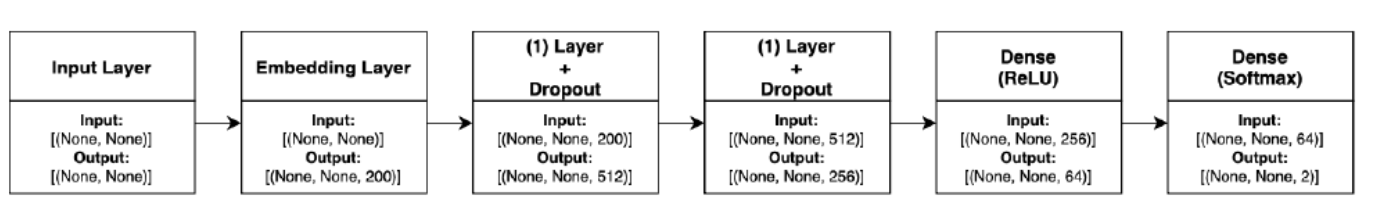
\includegraphics[width=0.45\textwidth]{images/bilstm_architecture.png}
  \caption{BI-LSTM architecture used in the model.}
  \label{fig:bilstm_architecture}
\end{figure}

\subsubsection{MLP}

To construct the MLP, RoBERTa-generated embeddings were initially loaded. The dataset was then partitioned into training and testing subsets, with an 80/20 split, respectively.

The primary consideration in designing the MLP architecture was determining the optimal number of dense layers and neurons. To this end, a manual cross-validation procedure was conducted to evaluate different architectural configurations. The hyperparameters explored included the number of hidden layers (1, 2, or 3) and the number of neurons in the first hidden layer (32, 64, or 128).

For architectures with more than one hidden layer, each subsequent layer contained half the number of neurons of its preceding layer. Based on validation performance, the best configuration consisted of two hidden layers: the first with 32 neurons and the second with 16 neurons, as illustrated in Figure~\ref{fig:mpl_layer_diagram}.


\begin{figure}[htbp]
    \centering
    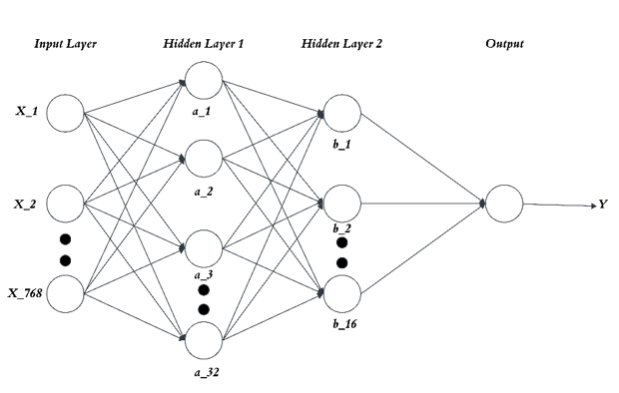
\includegraphics[width=0.8\linewidth]{images/MPL_layer_diagram.png}
    \caption{Diagram of the MLP layer architecture.}
    \label{fig:mpl_layer_diagram}
\end{figure}
 

\subsubsection{Fine-tuning methodology for RoBERTa}

To fine-tune the pretrained \texttt{twitter-roBERTa} model and adapt it to solve the classification task, we used the tokenized input data, which had not yet been embedded by the model. These data were split into 70\%, 15\%, and 15\% for the training, validation, and test sets, respectively, similar to the BI-LSTM architecture. 

Next, we created a three-layer classification head following the architecture shown in Figure~\ref{fig:roberta_finetune_architecture} \cite{liu2019roberta}. Dropout layers were added to prevent overfitting. This classification head was then integrated with the RoBERTa encoder, using the representation of the \texttt{[CLS]} token, which, as mentioned before, summarizes the input sequence.

With the full model ready, we froze the RoBERTa weights to train only the classification head. The training lasted 150 epochs, used batches of 32 samples, and employed the Adam optimizer, storing the checkpoints of the best-performing models. After this first stage, we evaluated the results and performed a second training stage, where all pretrained weights were unfrozen. This second stage was trained using a learning rate of 0.000001, the Adam optimizer, for 100 epochs, again with a batch size of 32.

To assess the best model from each training stage as well as the untrained model, we used precision, recall, F1-score, accuracy, and the confusion matrix.

\begin{figure}[htbp]
  \centering
  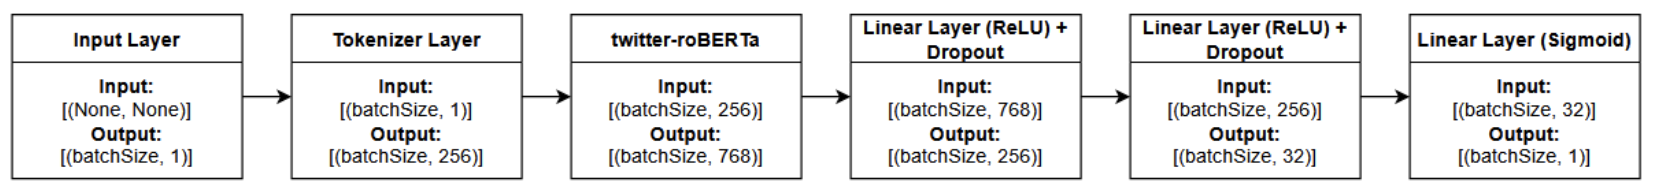
\includegraphics[width=0.45\textwidth]{images/roberta_finetune_architecture.png}
  \caption{Architecture used for fine-tuning twitter-RoBERTa.}
  \label{fig:roberta_finetune_architecture}
\end{figure}
